\documentclass[12pt]{article}
\usepackage{amsmath}
\usepackage{graphicx}
\usepackage[utf8]{inputenc}
\usepackage[T1]{fontenc}
\usepackage[french]{babel}
\usepackage{amsfonts,amsmath,amssymb}
\usepackage{float}
\usepackage{graphicx}
\usepackage{amsmath}
\usepackage{newunicodechar}
\usepackage[export]{adjustbox}
\usepackage[a4paper]{geometry}
\usepackage{fancyhdr}
\pagestyle{fancy}
\renewcommand\headrulewidth{1pt}
\fancyhead[L]{Documentation interactive dans les applis du rectorat}
\fancyhead[R]{Académie de Rennes}
\renewcommand\footrulewidth{1pt}
\fancyfoot[L]{Mouhyi MOUTARAJJI}
\begin{document}
\begin{titlepage}
	
    \vspace*{0.0 cm}
    \begin{flushleft}
    
    
\includegraphics  [scale = 0.6] {diagrammes/logo_Rectorat.jpg}
\includegraphics  [scale = 0.1] {diagrammes/lo.png}
    \end{flushleft}
    \textsc{96 Rue d'Antrain}\hspace{100 pt}\textsc{ UFR Informatique - Électronique }\\
    \hspace{20 pt}\textsc{35700 RENNES }\hspace{200 pt}\textsc{Campus De Beaulieu}\\
   \text{.} \hspace{289 pt}\textsc{35042 Rennes Cedex}\\
   \\
   \\
   \\
   \\
 	\centering   % Course Code
	\textsc{\large Master 2 Informatique}\\
		\textsc{\large Ingénierie Logicielle en alternance}\\
		\textsc{\large 2018/2019}\\
	\rule{\linewidth}{0.7 mm} \\[0.2 cm]
	\textsc{\large Documentation interactive dans les applications du rectorat}\\
	\rule{\linewidth}{0.2 mm} \\[0.2 cm]

	\centering   % Course Code
	\textsc{ Mouhyi MOUTARAJJI}\\
		\begin{flushleft} \large
		    \emph{Maîtres d'apprentissage:} \\
		    Annabel BOURDÉ, Annabel.Bourde@ac-rennes.fr\\
			Gaël SALAÜN , Gael.Salaun@ac-rennes.fr\\
			
			
		\end{flushleft}
	
\end{titlepage}


\newpage

\tableofcontents
~
\newpage

\section{Introduction}

J'ai réalisé mon alternance de Master 2 ingénierie logiciel au sein du rectorat de l'académie de Rennes du 09 septembre 2018 au 30 août 2019. J'ai intégré la DSII (Direction des Systèmes d'Information et de l'Innovation) et plus précisément le pôle DINAMO (Développement et INtégration en environnement Académique ou Mutualisé) encadré par Annabel BOURDÉ et Gaël SALAÜN. Ce pôle s'occupe généralement de développer et maintenir des applications web national utilisées par les chefs des établissement, les élèves  ou leurs parents et aussi des applications métiers dédiés aux employés du rectorat.\newline


Durant mon alternance, j'ai eu plusieurs mission toutes orientées sur les  applications Web, une de mes principales missions était d'intégrer un outil de documentation interactive dans les applications du rectorat. Le travail consistait à trouver une solution qui permet aux administrateurs des applications d'être autonomes et pouvoir rajouter la documentation sans utiliser du code informatique. Une autre mission était de réaliser une interface graphique, j'ai donc eu la chance de pouvoir développer aussi bien sur le Back-end que sur le Front-end.\newline   

C'était une première expérience en tant qu'apprenti dans une entreprise, cela m'a permis d'acquérir des nouvelles méthodes de travail comme l'agilité et de plus j'ai pu travaillé sur des des concepts innovants ainsi qu'utiliser des technologies et outils actuels.\newline


Dans un premier temps, j'établirai une bref présentation du service informatique du rectorat en présentant les multiples pôles qui existent et son organisation. Puis je présenterai plus en détail les objectifs de mon alternance ainsi que les méthodologies de gestion de projet que j'ai suivies et les outils que j'ai utilisés. Enfin j'expliquerai les travaux réalisés dans ma mission et je conclurai avec un bilan de mon alternance.

\newpage


   

\section{Contexte général}
\subsection{Rectorat de l’académie de Rennes}

Le rectorat de l'académie de Rennes est une circonscription administrative propre à l’Éducation Nationale.\\
Elle regroupe 4 directions des services départementaux de l'Éducation Nationale : 
Côtes d'Armor, Finistère, Ille-et-Vilaine et Morbihan. Chaque direction des services départementaux de l'Éducation Nationale est placée sous la responsabilité d'un inspecteur d'académie, directeur académique des services de l'Éducation Nationale. Son rôle au sein de ces départements est de gérer les personnels, les élèves, les moyens financiers, les examens... de tous les établissements scolaires, depuis la maternelle jusqu'au lycée.


\subsection{Organisation}
(TODO)

\subsection{Pôle DINAMO}

Au sein du rectorat, nous trouvons le pôle DINAMO (Développement et INtégration en environnement Académique ou Mutualisé), dans lequel je travaille en tant qu'apprentis et dont l'activité principale est le développement et l'intégration académiques. 


\begin{enumerate}
\item \textbf{Missions :}\\

\begin{itemize}
\item - Mettre en œuvre des services numériques académiques ou mutualisés.
\item - Réalisation des applications web et fournir des applications fiables, sécurisées et adaptées aux usages des utilisateurs. 
\item - Assurer la maintenance et l'évolution des projets.\\
\end{itemize}

\item \textbf{Effectifs :}\\
L’équipe de développement du pôle DINAMO est constituée d’Arnaud Rupin, responsable du pôle, ainsi que 6 développeurs informatiques (Albane GUIHOMAT, Annabel BOURDÉ, Gaël SALAÜN, Maïna DIRINGER, Marc BERHAUT et Vincent CARON). Voir figure 1\\

\end{enumerate}

\begin{figure}[H]
	\centering
 		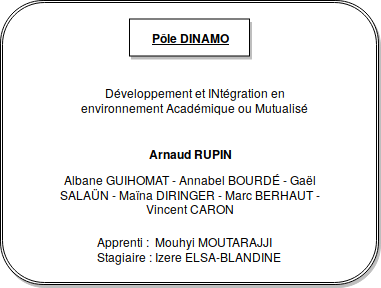
\includegraphics[width=1\textwidth]{diagrammes/PoleDinamo.png}
  		\caption{l'équipe du pôle DINAMO}
	\end{figure}


\subsection{Méthodes de travail}
\subsubsection{Méthodologie agile}

les nouveaux projets de l'équipe DINAMO fonctionnent en méthodologie agile sous forme de sprints qui varie de 2 à 4 semaines. Chaque équipe effectue un Daily-meeting afin d'échanger sur l'évolution des tâches à faire.

Durant un sprint, l'équipe embarque des nouvelles \textbf{User Story}\footnotemark. et réalise des nouvelles fonctionnalités ou corriger les erreurs et les bugs rencontrés lors des démos. Le lancement de chaque sprint se fait lors d'une réunion \textbf{sprint planning} dans laquelle toute l'équipe du projet est présente ainsi que le client. Ce dernier désigne les nouvelles \textbf{User Story} et des nouvelles fonctionnalités qu'il souhaite qu'elles soient rajoutées ou corrigées dans la prochaine version de l'application. 
\footnotetext{Un récit utilisateur, ou « user story »  en anglais, est une description simple d’un besoin ou d’une attente exprimée par un utilisateur et utilisée dans le domaine du développement de logiciels et de la conception de nouveaux produits pour déterminer les fonctionnalités à développer.}.

Durant mon alternance, j'ai eu la chance d'être inviter par mes maîtres d'alternances à assister plusieurs réunions des autres projets afin de voir le déroulement d'un projet agile. j'ai pu assister à un sprint planning, une rétrospective et une démo...    

Dans mon cas, j'étais le seul développeur dans mon projet, je faisais un Daily-meeting  tous les jours avec mes maîtres d'alternances pour que je puisse dire sur quoi je travaillais et leurs poser des questions en cas de blocages. L'administrateur des systèmes d'informations(ADSI) JOSSO Clément, qui est en même temps le Product Owner(PO) du projet, et mes maîtres d'alternances me conseillaient sur l'ordre des tâches à suivre lors des multiples réunions.   

\subsubsection{Communication}

Pour communiquer, l'équipe informatique utilise l'outil de messagerie instantané Rocket.Chat. Il permet de créer différents
channels pour chaque équipe, des channels de veille ont été également crées pour de la veille technologique.

Nous utilisons aussi l'outil Calendar (un outil développé par Oracle) qui permet d’organiser les réunions.  

\subsubsection{Dockerisation}

Le logiciel Docker permet de créer, déployer et exécuter des conteneurs de manière efficace. Un conteneur enveloppe l’application d’un logiciel dans une boîte invisible avec tout ce dont il a besoin pour s’exécuter.


Dans le pôle DINAMO, l'équipe utilise Docker Compose pour partager le même environnement de travail entre plusieurs personne et tout installer sur docker. Docker Compose est un outil qui permet de décrire et gérer  plusieurs conteneurs comme un ensemble des services inter-connectés.

Dans les projets sur lesquelles j'ai travaillés, nous avons utilisé Docker-compose pour déclarer tout les conteneurs dont nous avons besoin dans un fichier .yml  et nous démarrons l'ensemble des conteneurs en une seule commande \textbf{docker-compose up}. 

Dans le fichier docker-compose.yml, chaque conteneur est décrit avec un ensemble de paramètres qui correspondent aux options disponibles lors d’un docker run : l’image à utiliser, les volumes à monter, les ports à ouvrir...
 

\subsubsection{Versionning}

L'équipe informatique utilise Git sur la plateforme Gitlab hébergée par la Forge National comme gestionnaire de versions. 

\section{À propos du projet}

\subsection{Contexte et Problématique}

La DSII (Direction des Systèmes d'Information et d'Innovation et plus précisément l'équipe DINAMO utilise plusieurs façons pour documenter leur applications. La plupart du temps elle utilise une documentation écrite (Manuel Utilisateur), une chose qui ne rend pas facile aux utilisateurs de se documenter sur l'appli à cause de contrainte de temps. 


C'est pour cette raison que Monsieur JOSSO Clément,le product Owner du projet(PO), a voulu mettre en œuvre une documentation interactive dans l'application métier Solycee afin de faciliter l’accès de la documentation à ces utilisateurs et d'interagir directement avec la page web. Nous avons utilisé un outil nommé BootstrapTour pour réaliser cette documentation. 

Le besoin du client est d'avoir une application qui permet à l'ADSI(Administrateur Des Systèmes d'Informations) de créer la documentation directement à partir de sa page web et pouvoir l'améliorer au fur et à mesure des demandes des utilisateurs via une interface graphique rajouter dans le projet Solycee. 


Le but final du projet est de permettre aux ADSI d'être autonomes et de pouvoir rajouter la documentation dans leurs applications. Nous avons donc crée un web service(AppTour) qui permettra aux ADSI de rajouter la documentation et la sauvegarder. 
 
\subsection{Présentation de Bootstrap Tour : Une visite guidée interactive}
 
Bootstrap Tour est une librairie JavaScript permettant de présenter de façon assez simple l’application, l’avantage, comme pour toutes les librairies en fait, c’est qu’il y a déjà des bouts de fonctionnalités toutes faites, ce qui évite de réimplémenter le code. Bootstrap Tour est une implémentation qui sert à créer une visite guidée pour une application.

Le bénéfice de l'utilisation de Bootstrap Tour est immédiat pour les utilisateurs car elle présente les fonctionnalités de la page directement sur l'écran soit en lançant la documentation  dés l'ouverture de la page ou en appuyant sur un bouton pour déclencher cette documentation.\\
\textbf{Mis en œuvre et  Utilisation :}

Pour utiliser une visite guidée par Bootstrap Tour, il suffit juste de récupérer les bibliothèques et les sources dont nous avons besoin. La première étape est de construire un "Tour" qui accepte un bon nombre de paramètres dont le paramètre "Step" (étape). Ensuite il suffit de donner des étapes à notre tour, pour chaque étape il faut définir certain attribut : 

\begin{itemize}
\item \textbf{Élement: } Élément sur lequel vous désirez afficher votre popup. 
\item \textbf{Title: } Titre affiché sur la popup. 
\item \textbf{Content: } Message affiché dans le corps du popup.
\item \textbf{placement: } Permet d’indiquer dans quel sens vous désirez afficher la popup.
\end{itemize} 



\subsection{Architecture du projet}

Le projet se constitue d'une interface utilisateur qui est une application web (Solycee) et d'un Back-end qui est une API REST (AppTour) qui communique avec une base de données relationnelles. Voir figure 2.

\begin{enumerate}
\item \textbf{Technologies :}\\

\begin{itemize}
\item \textbf{Java: }Langage du développement du Back-end de Solycee. 
\item \textbf{Kotlin: }Langage du développement de l'API Rest AppTour. 
\item \textbf{Maven: }Construction des projets Java et Kotlin du Back-end.
\item \textbf{Spring: } Framework du développement du Back-end de Solycee.
\item \textbf{Spring Boot: }Framework d'infrastructure du Back-end AppTour.
\item \textbf{Spring Security: } Framework de sécurité de l'application Solycee et le web service AppTour.
\item \textbf{JavaScript,CSS,HTML,Bootstrap: } Développement du Front-end de Solycee.
\item \textbf{JUnit: } Framework de test des Back-end Solycee et AppTour. 
\end{itemize} 
\end{enumerate}

\begin{figure}[H]
	\centering
 		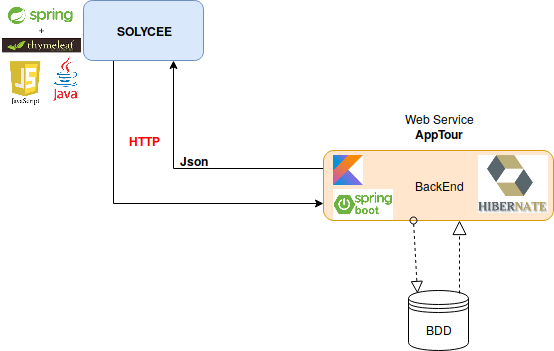
\includegraphics[width=1\textwidth]{diagrammes/ArchitectureGenerale.png}
  		\caption{Architecture du projet}
	\end{figure}


\section{Objectifs et missions de l'alternance}

\subsection{Solycee}

Solycee est une application métier créée par le pôle DINAMO et destinée à la gestion des offres et demandes de stages. Elle permet aux collèges et aux lycées d'inscrire leurs élèves dans des mini-stages proposés par les lycées.  

L'application serveur est réalisée en Java avec l'utilisation des composants du framework Spring.L'interface est codée avec le triplet HTML,CSS \& Javascript, les vues sont basées sur Thymleaf. 
\subsubsection{Architecture de l'application Solycee}

\begin{figure}[H]
    \centering
    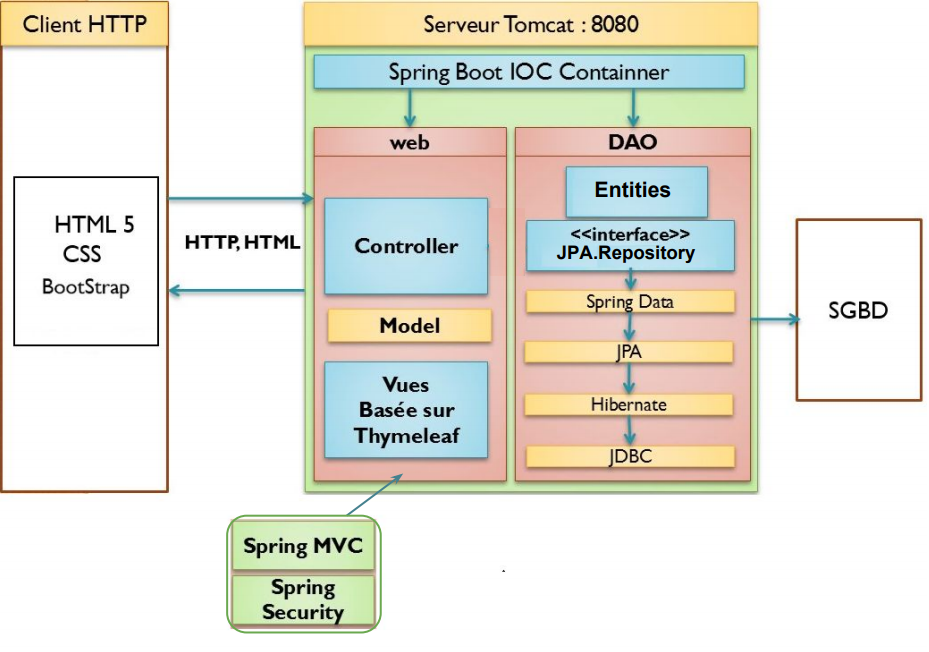
\includegraphics[width=0.9 \textwidth]{diagrammes/archiSolycee.png}
    \caption{Architecture logicielle de l'application Solycee }
\end{figure}

\subsubsection{Aspect technique}

Le projet est implémenté selon le patron de conception MVC et réalisé avec plusieurs technologies, la plupart de ces dernières sont open-source.L'application est implémentée avec un Back-end et un Front-end.

Le Back-end a été implémenté avec le framework Spring et le langage Java. Le coté interface (Front-end) a été réalisé avec le moteur de template Thymeleaf. 

Voici maintenant une présentation plus précise sur les principaux outils utilisés:\newline

\textbf{Spring:} Spring est un framework libre pour construire et définir l'infrastructure d'une application java dont il facilite le développement et les tests. Le concept fondamental du Spring, qui fait sa force, est l'injection des dépendances (dependency injection).\newline

\begin{itemize}
	\item \textbf{Spring MVC} : Spring MVC est un framework qui permet d’implémenter des applications selon le design pattern MVC. Spring MVC se base sur le principe décrit par le schéma ci-dessous :\newline
	

\begin{figure}[H]
	\centering
 		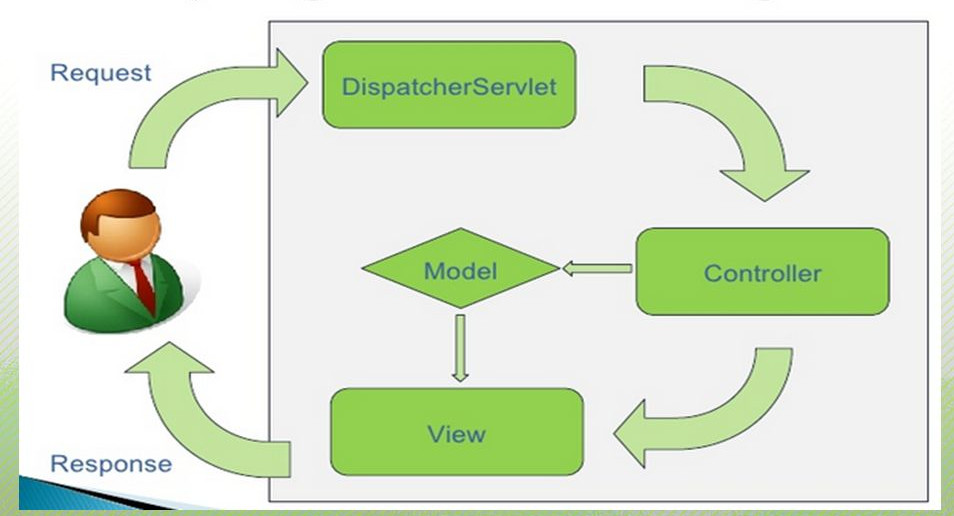
\includegraphics[width=1\textwidth]{diagrammes/mvc2.jpg} 
  		\caption{Schéma du patron de conception MVC}
	\end{figure}
	
	\item \textbf{Spring Security }: Spring Security est un Framework de sécurité léger qui fournit une authentification et un support d’autorisation afin de sécuriser les applications Spring. \newline
\end{itemize} 

\textbf{Kotlin:} Kotlin est un langage de programmation orienté objet et fonctionnel, il a plusieurs avantages, voici les plus importants :
\begin{itemize}
\item \textbf{Typage statique: } Kotlin est un langage de programmation à typage statique. Cela signifie que le type de chaque variable et expression est connu au moment de la compilation.
\item \textbf{Sécurisé: } Kotlin est sécurisé. Il évite les exceptions NullPointerExceptions les plus redoutées en prenant en charge la nullabilité dans le cadre de son système de types.
\item \textbf{Facile à apprendre: } La syntaxe ressemble beaucoup à la syntaxe Java.
ect.
\end{itemize} 
\textbf{Maven:} Maven est un outil de construction de projets (build) open source développé par la fondation Apache. Il permet de faciliter et d'automatiser certaines tâches de la gestion d'un projet Java. Le but est de produire un logiciel à partir de code source en optimisant les tâches à réaliser. Il est facile à configurer.\newline

\textbf{Hibernate: } Hibernate est un framework open source de type ORM (Object Relational Mapping) qui permet de faciliter le développement de la couche persistance d'une application. Il permet donc de représenter une base de données en objets Java et vice versa.

\textbf{Thymeleaf:} Thymeleaf est un Java XML/XHTML/HTML5 Template qui apporte le concept de templates naturels en utilisant des attributs HTML spécifiques. Ce framework apporte aussi une séparation entre l'affichage et le contenu.\\

Thymeleaf s’intègre très facilement dans un projet Spring et permet de diffuser XHTML/HTML5 sur la vue des applications WEB.


\subsubsection{Travail réalisé}


Dans le projet Solycee, j'ai principalement travaillé sur la partie Front-end. J'ai réalisé plusieurs tâches soit en rajoutant des nouvelles vues et des nouveaux composants dans les pages web et/ou en rajoutant des nouvelles fonctionnalités sur les composants existants.

Le projet a été développé par l'équipe Dinamo. Avant de commencer à réaliser les tâches demandées, il était nécessaire de procéder un travail  de lecture du code implémenté et de la compréhension de ce dernier en posant des multiples questions à mes maîtres d'alternances. Il m'a fallu aussi comprendre l'architecture du projet ainsi que les technologies utilisées. 

Une fois que le code était compréhensible et j'ai acquis toutes les informations importantes sur le projet, j'ai commencé à réaliser les tâches demandées.

J'ai commencé par manipuler Bootstrap Tour sur l'application Solycee en rajoutant le code de la librairie dans le front de Solycee (code en javascript avec les étapes souhaités). Suite à une demande de l'ADSI de Solycee nous avons pu réaliser une première version en utilisant Bootstrap Tour. Un tour est défini dans un fichier JavaScript et il est composé de différent étapes. Bootstrap tour permet d'afficher l'étape du tour et aussi passer à l'étape suivante ou précédente ainsi que arrêter le tour avec le bouton "Fin"(Voir Figure 5). Pour lancer la documentation faut juste exécuter  2 méthodes dans le fichier Javascript, init et star. 
\begin{figure}[H]
	\centering
 		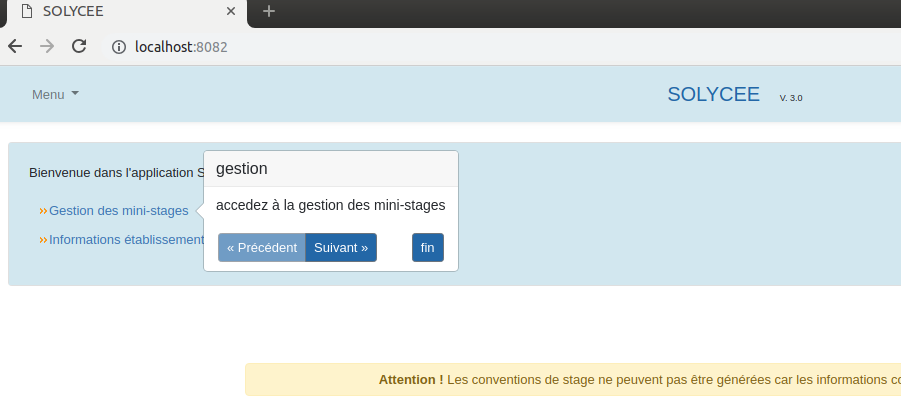
\includegraphics[width=1\textwidth]{diagrammes/exemple_Tour.png} 
  		\caption{Exemple d'une étape de Bootstrap Tour}
	\end{figure}

\begin{enumerate}
\item \textbf{Ajout de fonctionnalité :}\\
Voici maintenant une présentation plus précise des fonctionnalités rajoutées : 

\begin{itemize}
\item - L'ajout d'une modale pour prévenir les utilisateurs de la présence d'un bouton aide pour déclencher la documentation interactive.Voir Figure 6

\begin{figure}[H]
	\centering
 		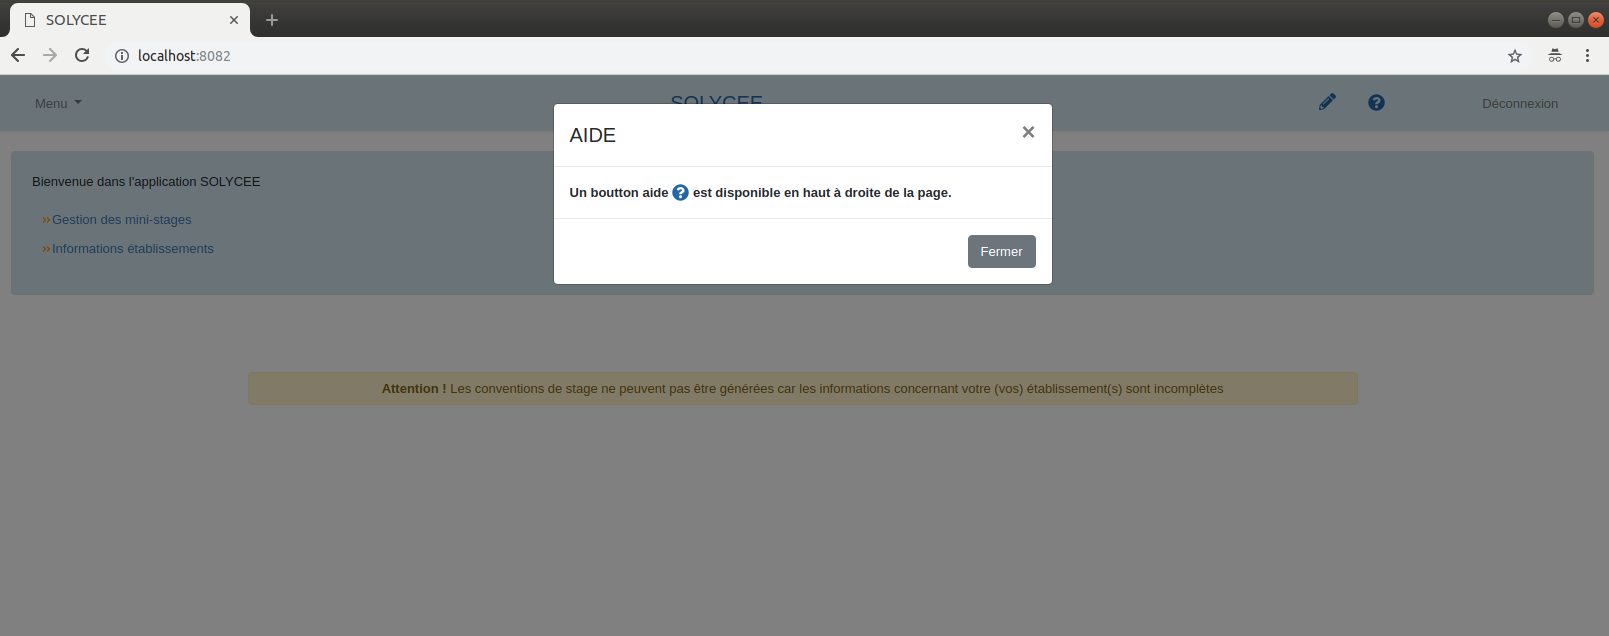
\includegraphics[width=1\textwidth]{diagrammes/aide_modal.png}
  		\caption{Page d'accueil Solycee}
	\end{figure}
Pour que cette modale n'apparaît qu'une seule fois chez les utilisateurs de l'application. Nous avons fait en sorte qu'elle ne s'affiche que si l'utilisateur consulte l'application Solycee pour la première fois. \\ 


\underline{Mise en oeuvre} :
Pour réaliser cette tâche, j'ai dû ajouter une modale qui est un composant Bootstrap qui s'affiche à la première connexion de l'utilisateur à l'application. Cette modale n'apparaît pas une deuxième fois. \\ 

   
\item - Déclencher la documentation interactive en appuyant sur un bouton: Dans la première version, la documentation se déclenchait dés que l'utilisateur arrive sur la page de l'application et cela peut être répétitif pour l'utilisateur. Dans le cas présent, la documentation s'exécute seulement en cliquant sur un bouton. \\ 

\underline{Mise en oeuvre} :
Rajout du Bootstrap Tour : Il s'agit de l'ajout d'un bouton 
\includegraphics[width=5mm,scale=0.5]{diagrammes/Bouton_aideDispo.png} sur toutes les pages web de l'application. En appuyant dessus ça déclenche les pop-ups  de Bootstrap tour. 


La mis en place de Bootstrap Tour dans un ficher Javascript était une façon simple non compliqué pour lancer une documentation interactive. Il suffit juste de rajouter des Tours et des Steps dans le fichier JS, donc il faut aller chercher et modifier dans le code, une manipulation qui peut être compliqué des fois.

Nous avons donc créé un web service AppTour où sont sauvegarder les Tours et les Steps. L'application Solycee communique avec ce web service pour récupérer les informations et la documentation. \\ 

\item - Récupérer La documentation d'une page web de l'application Solycee: Il suffit de faire un appel au Web service AppTour. \\   
 
\underline{Mise en oeuvre} :
- Chaque page HTML(Vue) de l'application Solycee a un identifiant qui correspond à l'Id de son corps "Body".

- Un fichier JavaScript "tourLoader" est importé dans toutes les vues de Solycee.

- Nous interrogeons le Web service AppTour avec une requête Ajax en passant en paramètre le nom de l'application et l'identifiant de la page courante. La requête vérifie s'il existe de la documentation pour l’identifiant concerné. 

- Si la requête renvois un fichier json qui contient les tours et les étapes à déclencher avec Bootstrap Tour, l'utilisateur peut exécuter une documentation interactive en cliquant sur le bouton 
\includegraphics[width=5mm,scale=0.5]{diagrammes/Bouton_aideDispo.png}. Voir Figure 5.    

- Dans le cas où il n'existe pas de documentation sur la page web, le bouton affiché est gris et titré par une phrase "Aide non disponible pour cette page". Voir Figure 7 \\
\begin{figure}[H]
	\centering
 		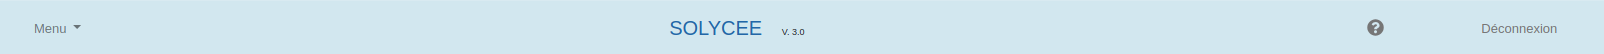
\includegraphics[width=1\textwidth]{diagrammes/aideNonDispo.png} 
  		\caption{Pas de tour disponible dans cette page Web }
	\end{figure}
    
\item - Rajouter un mode d'édition pour les ADSI: Jusqu'à maintenant, les ADSI ne pouvaient pas rajouter la documentation sauf s'ils rajoutent des données en dur dans la base de données, chose qui n'est pas facile. Pour cette cela, nous avons créé un mode édition dans l'application Solycee qui est présenté par une interface graphique et elle  permet de rajouter la documentation.\\


\underline{Mise en oeuvre} : \\
- Nous avons rajouter le bouton
\includegraphics[width=5mm,scale=0.5]{diagrammes/Bouton_modeEdition.png} dans toutes les pages web de l'application Solycee qui est titré par une  phrase "Veuillez cliquer ici pour passer en mode édition".

- En appuyant sur le bouton 
\includegraphics[width=5mm,scale=0.5]{diagrammes/Bouton_modeEdition.png} les ADSI passe en mode édition pour rajouter la documentation souhaité sur n'importe quel composant de la page web.Nous affichons un champs sur l'interface pour prévenir les ADSI qu'ils sont passés en mode éditions.Voir Figure 8.

\begin{figure}[H]
	\centering
 		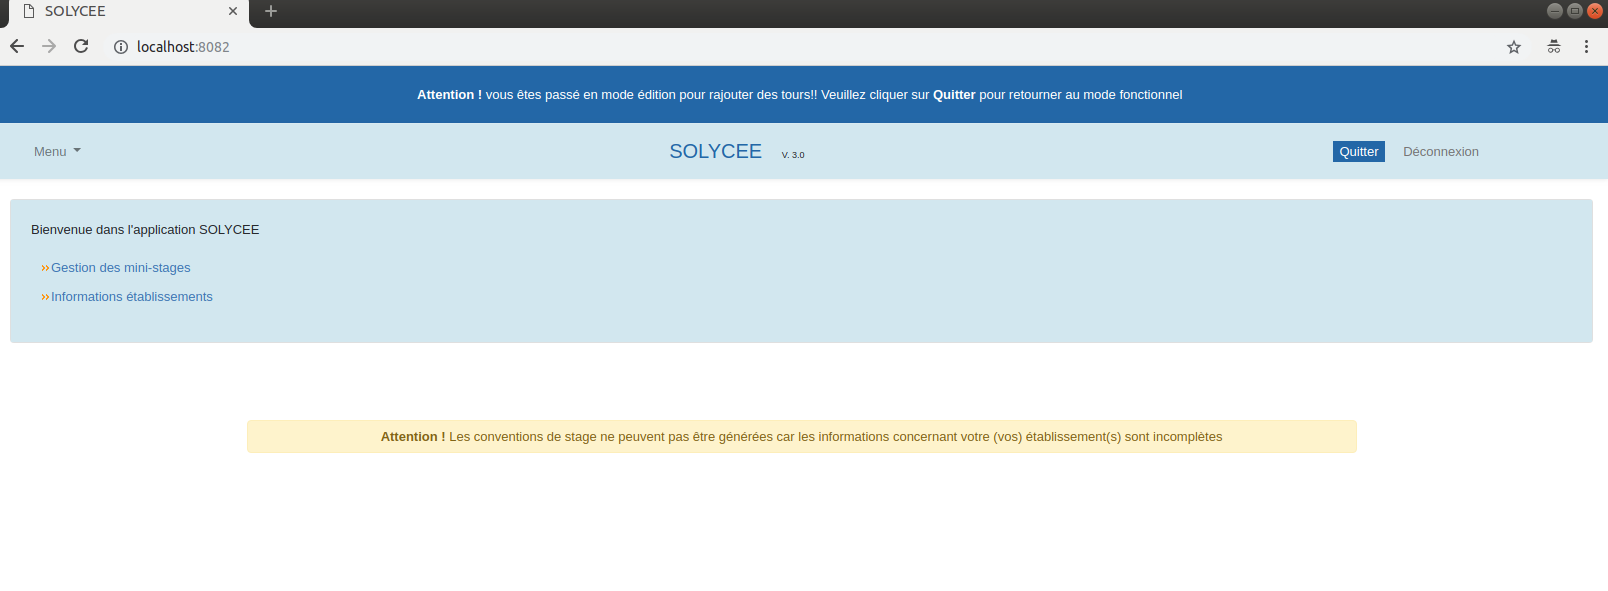
\includegraphics[width=1\textwidth]{diagrammes/mode_edition.png} 
  		\caption{Page d'accueil en mode édition}
	\end{figure}
 

 Ce mode consiste à rester sur la même page web où il se trouvait l'ADSI mais le comportement des composants(boutons, url,logo,etc...) de cette page change et ne fonctionne plus comme le mode normal. 

Si l'ADSI appuie sur un composant de la page alors qu'il est en mode édition, cela affiche une modale qui contient plusieurs composants(Titre,Élément,Contenu...) créés en HTML et CSS.

\begin{itemize}
\item \textbf{Élement: } Id de l'élément sélectionné. 
\item \textbf{Title: } Titre affiché sur la popup. 
\item \textbf{Content: } Message affiché pour expliquer le fonctionnement du composant appuyé.  
\end{itemize}
\item - Pour sécuriser un minimum le mode édition, nous avons fait en sorte que seuls les ADSI peuvent rajouter la documentation et non les utilisateurs et ils sont les seuls à accéder à ce mode.\\ 


\underline{Mise en oeuvre} : \\
- Quand l'utilisateur se connecte sur l'application, nous récupérons son nom complet.

- Nous interrogeons ensuite le Web service AppTour en utilisant  Srping-RestTemplate\footnotemark, nous envoyons une requête HTTP en passant en paramètre le noms complet d'utilisateur et le libelle de l'application. Si l'utilisateur est présent dans la table Personnel de AppTour, il est ADSI et dans ce cas il a le droit d'accéder au mode édition. Dans le cas inverse, l'utilisateur n'a pas le droit à ce mode et le bouton 
\includegraphics[width=5mm,scale=0.5]{diagrammes/Bouton_modeEdition.png} ne s'affiche pas.
\footnotetext{Spring RestTemplate est un Framework de Spring qui permet d'établir une communication entre un client et un serveur REST, ceci grâce aux requêtes HTTP.}.\\


\item - Remplir les champs de la modale : Quand les ADSI passent en mode édition et en appuyant sur un composant de la page web, la modale s'affiche qui permet de rajouter ou modifier la documentation. Ensuite, nous remplissons les champs de la modale dans le cas où il existe une documentation pour ce composant. \\

\underline{Mise en oeuvre} : 

- En appuyant sur un composant de la page, nous envoyons une requête Ajax au Web service AppTour pour récupérer l'étape dans le cas SI elle existe. Nous passons en paramètre l'Id du l'élément appuyer ainsi que id du tour de la page web où il se trouve l'ADSI. 

- Si l'étape existe dans la table Step de AppTour,nous récupérons l'objet et puis nous remplissons les champs par les données récupérées(Title \& content).Voir Figure 9.

\begin{figure}[H]
	\centering
 		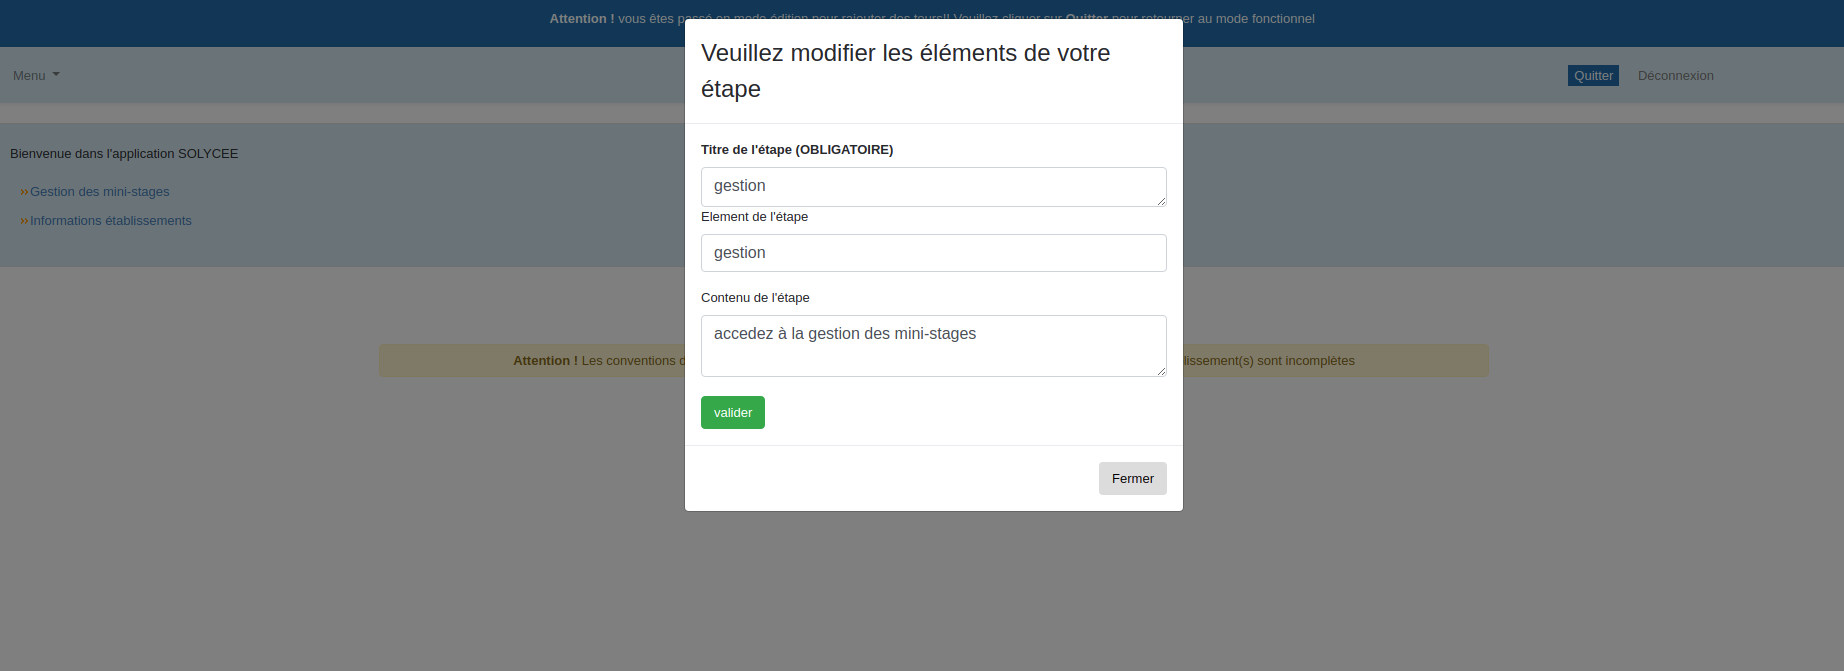
\includegraphics[width=1\textwidth]{diagrammes/Modal_gestion.png} 
  		\caption{une documentation existe déjà pour le lien Gestion des mini-stages}
	\end{figure}

- Dans le cas où il n’existe pas de documentation pour l'élément sélectionné, nous laissons les champs vides.\\ Voir Figure 10.

\begin{figure}[H]
	\centering
 		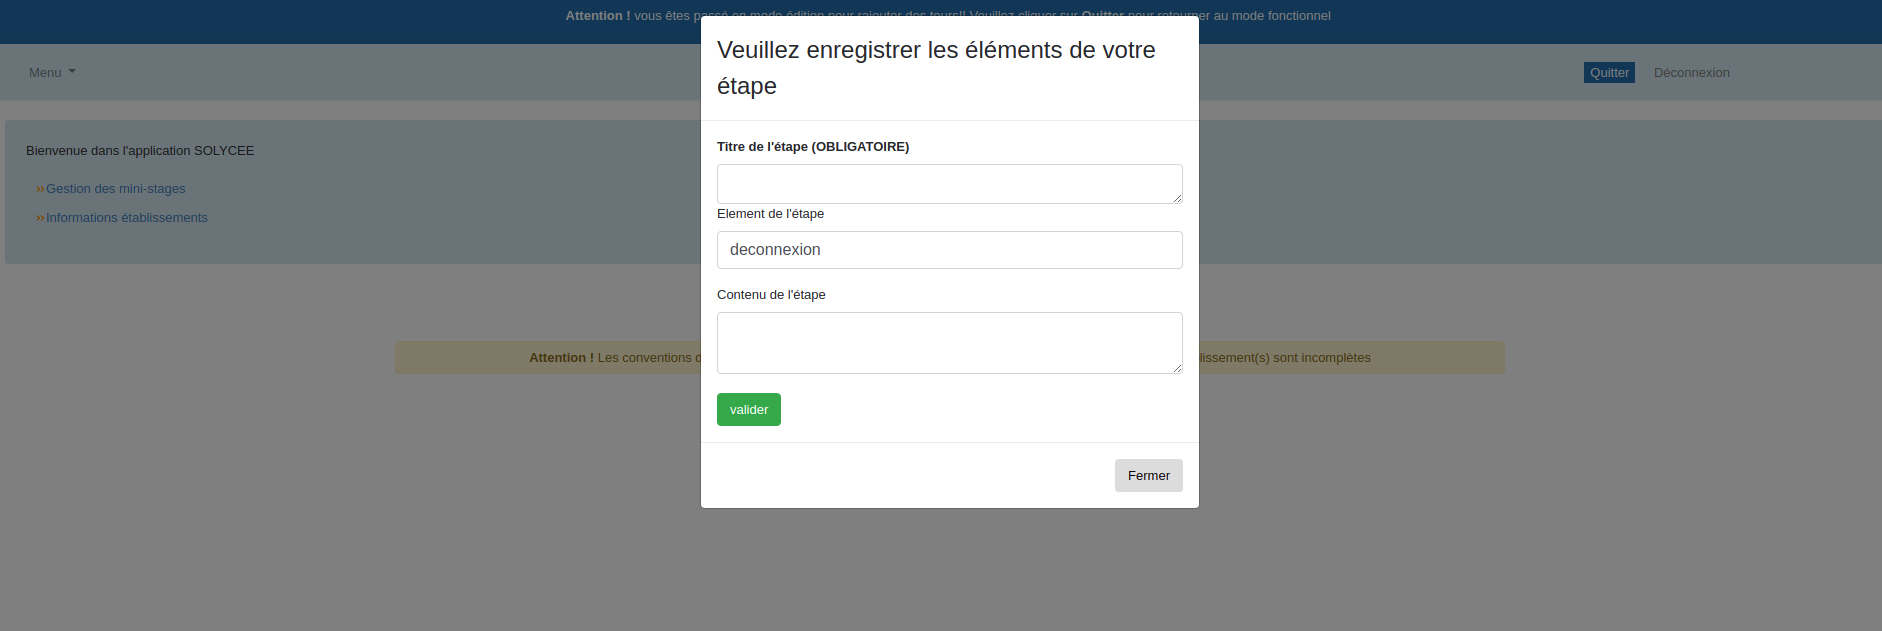
\includegraphics[width=1\textwidth]{diagrammes/Modal_Deconnexion.png} 
  		\caption{Pas de documentation pour le bouton Déconnexion}
	\end{figure}

\item - Rajouter ou modifier la documentation : Quand l'ADSI est en mode édition, il peut soit rajouter la documentation pour un composant de la page web dans le cas où il n'existe pas de documentation pour ce dernier, soit la modifier dans le cas où elle existe. 
 
\underline{Mise en oeuvre} : 

- Après que nous interrogeons le Web service AppTour sur la présence de la documention pour le composant appuyer, si elle est présente nous remplissons les champs et l'ADSI peut la modifié en changeant le contenu de l'étape ou son titre. Le bouton valider de la modale permettra alors d'envoyer une requête Ajax (PUT) au Web service pour stocker les  modifications faite sur l'étape. 

- Dans le cas où elle n'existe pas de documentation pour l'élément appuyé, l'ADSI peut remplir les champs vides(Mettre un titre à la nouvelle étape et un contenu pour expliquer le fonctionnement de l'élément). Le bouton valider permet cette fois d'envoyer une requête Ajax (POST) pour rajouter la nouvelle étape dans la table Step.  

\end{itemize}

\end{enumerate}

\subsection{AppTour}   

Comme expliquer plus haut, au début nous avons commencé par manipuler Bootstrap Tour en rajoutant du code JS de la librairie. Chose qui n'est pas facile et pas efficace. Pour cette raison, nous avons créé le Web service AppTour afin de permettre aux ADSI des applications de stocker leurs documentations. 

AppTour est un Web service qui permet aux ADSI de rajouter ou modifier les étapes de leur documentation interactive (Bootstrap Tour). 
API Rest AppTour est une application Spring Boot codée en langage Kotlin, nous avons implémenté plusieurs Endpoint afin stocker leurs documentations. 


\subsubsection{Architecture de l'API AppTour}



Le Back-end AppTour, c’est la partie du code qui est exécutée par le serveur, il s'agit d'un serveur qui fourni une API Rest gérant la persistance des données et la logique de l'application. 

L'architecture du Web service AppTour est similaire avec les nouveaux Webs services implémentés par le pôle Dinamo, j'ai essayé de respecter cette architecture pendant mon développement. 

Le Back-en Apptour se décompose de plusieurs couches: \newline

\textbf{(TODO)!!!}

Une couche Repository/DAO: Repositories sont des interfaces héritant de l'interface Repository. L'objectif de ces interfaces consiste à rendre la création de la couche d'accès aux données (requêtes SELECT, UPDATE...) plus rapide.\newline


Une couche Service: Elle permet de séparer les opérations effectuées par le contrôleur et celles qui concernent le modèle des données. Toute action devrait passer par cette couche.\newline


Une couche Contrôller: Il s'agit de l'API qui permet de répondre à toutes les requêtes envoyées par le client. 


\begin{figure}[H]
	\centering
 		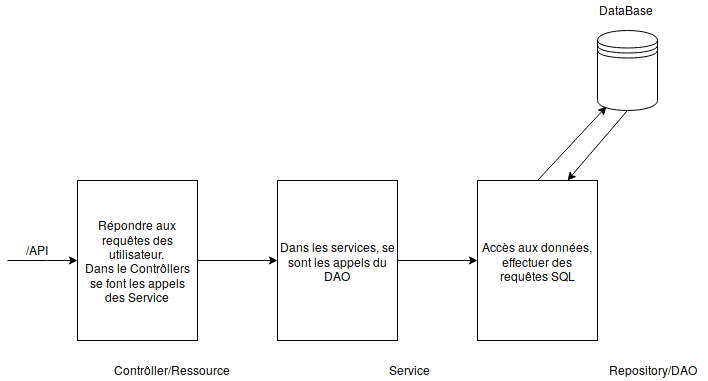
\includegraphics[width=1\textwidth]{diagrammes/ArchitectureProjet.png}
  		\caption{Arichtecture Back-end d'une application web}
	\end{figure}
	



\subsubsection{Aspect technique}
(TODO)!!!
 Le projet AppTour était initialiser par l'alternant de l'année dernière. j'ai commencé par la relecture du code et la compréhension de l'existant. L'application a été implémenté en Kotlin qui est un langage de programmation orienté objet et fonctionnel, avec un typage statique qui permet de compiler pour la machine virtuelle Java et JavaScript et Spring boot qui est un framework utilisé afin de faciliter la configuration d'un projet Spring et de réduire le temps alloué au démarrage d'un projet. plusieurs autres technologies était utilisées dans ce projet : 
 
\begin{itemize}
\item Maven :  Est un outil de gestion et d'automatisation de production des projets logiciels Java en général et Java EE en particulier. Il est utilisé pour automatiser l'intégration continue lors d'un développement de logiciel.

\item JUnit : Pendant mon développement de l'API AppTour, j'ai utilisé la méthode du TDD(Test Driven Development),le développement piloté par les tests. j'ai utilisé le framework JUnit pour implémenter les tests unitaires afin d'assurer la maintenance et l'efficacité de l’application.

\item Git : Est un logiciel de gestion de versions décentralisé. Il permet de sauvegarder les fichiers en gardant la chronologie de chaque sauvegarde.

\item L'API AppTour a été réalisé de la même manière que les autres applications du rectorat. Il existe plusieurs couches. Une couche service pour implémenter tous les services dont nous avons besoin, une couche controller pour construire l'API utilisée par le Front Solycee et qui sera utilisée par d'autres applications dans le futur, il existe d'autres couches afin de créer une application similaire aux autres applis du rectorat.

\end{itemize}

\subsubsection{Travail réalisé}
(TODO)!!!
Dans le projet AppTour, j'ai travaillé sur la réalisation d'une API web (Le back-end pour le bootstrapt), j'ai développé plusieurs Web Services qui permets de rajouter ou modifier les étapes des tours ainsi que faire des recherches pour vérifier l’existence des tours. 

Comme noté plus haut, le projet AppTour était initialiser par l'alternant de l'année dernière en créant les tables (Entity). Il existait deux tables, une table Tour et une table Step. j'ai commencé donc par la relecture du code existant et la modification des tables.
Ensuite, Nous avons travaillés avec mes maîtres d'alternance sur l'architecture du projet.

Une fois que le code et le travail demandé était compris et acquis, j'ai commencé par implémenté du code nécessaire pour réaliser les web services dont nous en avons besoin. Voici une présentation plus précise de toutes les tâches réalisées:   

\begin{itemize}

\item rajouter des éléments dans les tables par exemple Storage dans l'entité Tour qui est un booléen et qui permet de configurer si on veut stocker les tours dans l'historique ou pas ou encore la variable Ordre dans l'entité Step qui un entier et qui permet de donner un ordre pour chaque step.  
\item Créer toutes les classes DTO afin de les utiliser dans les requêtes  pour envoyer ou récupérer des données.

\item Implémenter les classes Repositories qui permettent de faciliter l'accès  ou le stockage des données dans la base.

\item Créer des classe Mapper qui permettent de convertir un objet Dto à un objet normal ou l'inverser. Par exemple passer d'un objet TourDto à un objet Tour il suffit d'appeler la méthode tourDtoToTour et qui prend en paramètre un objet tourDto : TourDto.  

 \begin{figure}[H]
	\centering
 		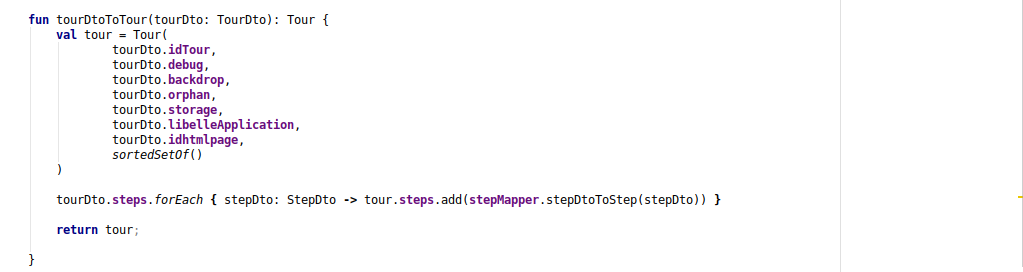
\includegraphics[width=1\textwidth]{diagrammes/Exemple_tourDtoToTour.png} 
  		\caption{Exemple d'une méthode de la classe TourMapper}
	\end{figure}

\item La réalisation de l'API et tout les services Web, il s'agit d’implémenter des classes contrôllers qui consomme toute les méthodes qui se trouvent dans les classes services. Il existe plusieurs types de services web: 
\begin{itemize}
\item Des méthodes GET : Pour la récupération des données de la base dans le cas où elles existent. Par exemple "retrieveTourByIdHtmlPage" ou encore "getStepByElementandIdTour".

\item Des méthodes POST : Pour stocker des nouveaux objets dans la bas de données. Par exemple "saveTour" ou encore "saveNewStep".

\item Des méthodes PUT : Pour mon projet, j'ai du m’en servir  d'une méthode "updateStep" qui permet au utilisateurs de modifier une étapes qui existe déjà.

\end{itemize}
\item L'implémentation des classes Services: Toutes les actions effectuer le contrôller doivent passer par les classes services. 

Il existe une classe TourService: Dans cette classe, j'ai réalisé plusieurs méthodes qui permettent à stocker ou récupérer des Tours de la base données : 
\begin{itemize}
\item  retrieveTourByLibelleAndIdHtmlPage : Elle permet à récupérer un tour en passant en paramètre nom d'une application et l'identifiant de la page HTMl. 

\item saveTourWithLibelleAndIdHtmlPage : Elle permet à stocker un tour dans la base de données en donnant le nom de l'application et l'Id de la page HTML. 

\item updateTour : Elle permet à modifier un tour existant dans la base données en donnant des nouveaux paramètres. 
\end{itemize}

Il existe aussi une classe StepService : Dans cette classe, j'ai réalisé plusieurs méthodes qui permettent à stocker ou récupérer des Step de la base données : 
\begin{itemize}

\item  findStepByElementandIdTour : Elle permet de récupérer un Step en passant en paramètre l'élément rechercher et l'identifiant du tour.

\item saveStep : Elle permet à stocker un Step dans la base de données.

\item findOrdreMax : Elle permet de lister tout les step d'un tour par ordre croissant.  
\end{itemize}
\end{itemize}
\subsection{Partie Sécurité}
\subsubsection{Permettre seuls aux administrateurs de modifier les tours}

Pour permettre seuls aux administrateurs de l'application Solycee de passer en mode édition  et pouvoir rajouter et/ou modifier des tours, j'ai créé une nouvelle table(Entité) Personnel dans l'API AppTour, cette table contient un identifiant et libellé de l'application, les personnes présentes dans la tables Personnel sont des administrateurs de leurs applications. Après j'ai commencé à réaliser les classes nécessaires dans la même architecture que les tables Tours et Step. J'ai implémenté donc une classe PersonnelDto et puis une classe PersonnelMapper qui permet de passer d'un objet Personnel à un objet PersonnelDto ou l'inverse(d'un objet PersonnelDto à un objet Personnel), ensuite j'ai créé la classe PersonnelService pour pouvoir implémenter les méthodes utilisées par la classe PersonnelController.Enfin, J'ai implémenté un service qui permet de faire une recherche dans la table Personnel et vérifier la présence de la personne en donnant son identifiant (Nom + Prénom) et aussi le libellé de l'application. 


En laçant l'application Solycee, je récupère l'identifiant de la personne connecté (Toute personne connecté a un identifiant (Nom + Prénom)) et puis j’envoie une requête à l'API AppTour pour vérifier si la personne connecté est présente dans la table Personnel. Dans le cas ou la requête renvoie une réponse positive (200 Succès), j'affiche le bouton qui permet aux admins de passer en mode édition, dans le cas contraire le bouton 
\includegraphics[width=5mm,scale=0.5]{diagrammes/Bouton_modeEdition.png} ne s'affiche pas. 



\subsubsection{Sécuriser l'API}


Après avoir réaliser toutes les tâches demandés par le PO(Product Owner), il voulait mettre les nouvelles fonctionnalités rajoutées en production pour avoir un avis des utilisateurs. Mais avant de les mettre en prod fallait sécuriser l'API Apptour ainsi que s'assurer que les personnes qui voudraient envoyer des requêtes à l'API ont les droit de réaliser ces requêtes et ils sont administrateurs de l'application. Nous avons donc décidé de sécuriser les échanges entre le client (Solycee) et l'API AppTour. 

Le premier travail a commencé par faire des recherches par rapport à la façon dont nous allons sécuriser les applications.Un sujet de recherche du rectorat était de pourvoir intégrer la plateforme Keycloak pour l'authentification des utilisateurs dans les applications. Solycee était une occasion pour commencer les recherches sur ce sujet.  Nous avons décidé de mettre en place une couche d'authentification basé sur OAuth 2.0 qui permet d'autoriser une application web (ou un logiciel) à utiliser une autre API sécurisé, et nous avons utilisé Keycloak localement pour s'authentifier et obtenir un Token JWT pour chaque utilisateurs de l'application.  
\includegraphics[width=30mm,scale=0.5]{diagrammes/logo_Keycloak.jpeg}  

La première étape était  d'installer un serveur Keycloak localement qui permettra par la suite de faire des tests. Keycloak  est un logiciel open source permettant l'authentification unique avec la gestion des identités et des accès, destiné aux applications et services modernes. Pour la configuration de keycloak, il suffit juste de fournir un fichier  royaume(Realm) ainsi qu'un fichier utilisateurs(User) pour renseigner les utilisateurs  avec leur identifiants et leurs mots de passe (Voir annexes pour un exemple des fichiers Realm et User)

Le fonctionnement de Keycloack nécessite  une configuration. IL faut déclarer plusieurs données : 
\begin{itemize}
\item Utilisateurs : Ils sont des entités pouvant se connecter à votre système
\item Rôles : ils identifient un type ou une catégorie d’utilisateur ( Admin, user, …)
\item Groupe : permet de gérer un groupe d’utilisateur
\item Royaumes (realms): un domaine qui gère un ensemble d’utilisateurs, d’informations d’identification, des rôles et des groupes.
\item Clients : ils sont des entités pouvant demander à Keycloak d’authentifier un utilisateur ( comme des applications )
\end{itemize}

Après l’authentification, nous obtenons un Identity token qui fournit des informations d’identité sur l’utilisateurAccess token : un token pouvant être fourni dans le cadre d’une requête HTTP autorisant l’accès au service invoqué.

En suite, j'ai fait des recherches pour trouver une libraire JavaScript qui permet à utiliser keycloak pour l'authentification. Pendant mon développement j'ai utilisé deux librairie JavaScript différentes mais le fonctionnement était le même. J'ai commencé par implémenté la librairie KeycloakJS et par la suite j'ai utilisé la librairie Oidc-clientJS pour permettre aux administrateurs de se diriger à une plateforme d'authentification, dans mon cas c'était Keycloak pour tester la librairies. Voici la plateforme d'authentification Keycloak: 
 \begin{figure}[H]
	\centering
 		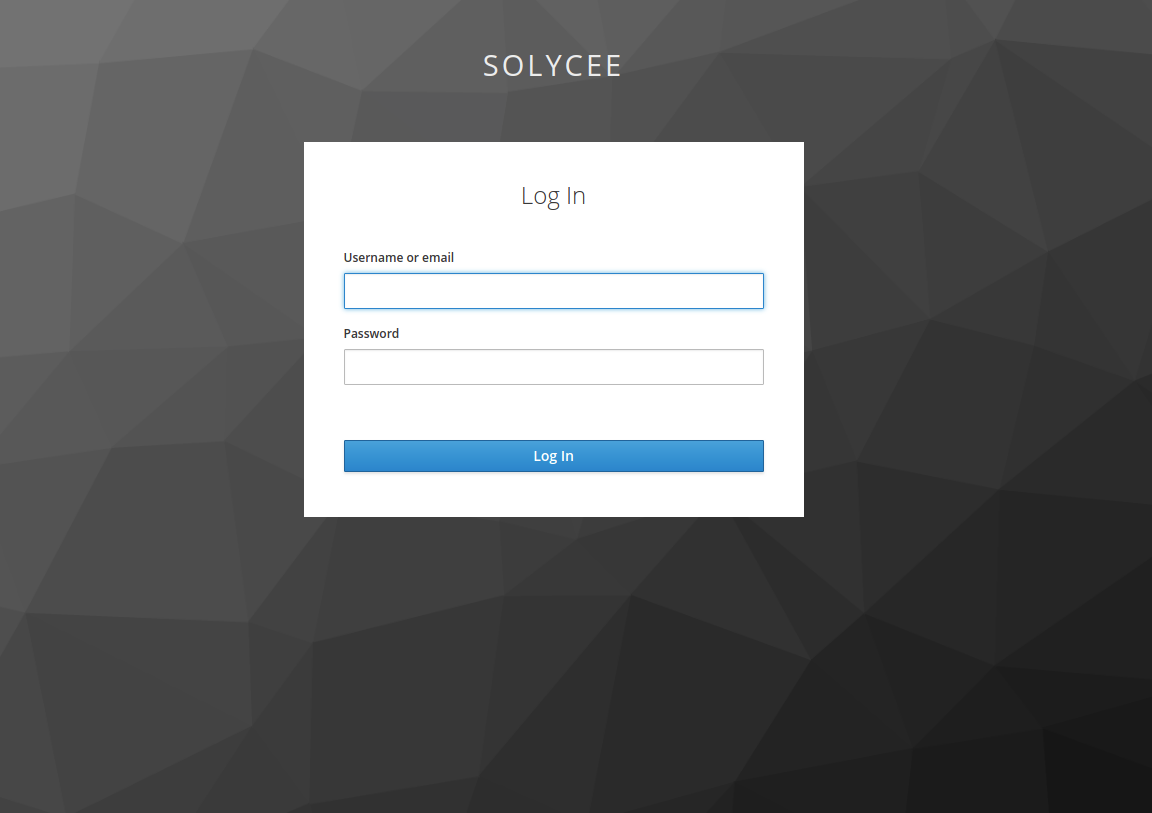
\includegraphics[width=1\textwidth]{diagrammes/authentification_keycloak.png} 
  		\caption{Authentification avec OpenID et Keycloak }
	\end{figure}

\newpage
\section{Annexes}

\end{document}
